\documentclass[conference]{IEEEtran}
\IEEEoverridecommandlockouts
% % The preceding line is only needed to identify funding in the first footnote. If that is unneeded, please comment it out.
% \usepackage{cite}
\usepackage{amsmath,amssymb,amsfonts}
\usepackage{algorithmic}
\usepackage{graphicx}
\usepackage{textcomp}
\usepackage{xcolor}
\usepackage{csquotes}
\usepackage[acronym, toc, nonumberlist]{glossaries}
\usepackage[style=ieee, backend=biber, defernumbers=true, maxcitenames=2, mincitenames=1, urldate=iso, date=iso, seconds=true, url=true]{biblatex}
\usepackage{float}	% For placing figures in minipages
\usepackage{fontawesome}
\usepackage{booktabs}
\usepackage{enumitem} % Add this line to the preamble of your document for custom numbering
\usepackage[hidelinks]{hyperref}

\hypersetup{
pdfnewwindow=True,
}

\def\BibTeX{{\rm B\kern-.05em{\sc i\kern-.025em b}\kern-.08em
    T\kern-.1667em\lower.7ex\hbox{E}\kern-.125emX}}

\setcounter{biburllcpenalty}{7000}
\setcounter{biburlucpenalty}{8000}
    
\makeatletter
\renewcommand\IEEEkeywordsname{Keywords}
\makeatother
\usepackage{xpatch}
\xpatchcmd\IEEEkeywords{---}{-}{}{}

\makeatletter
\renewcommand{\fnum@figure}{Figure~\thefigure}
\makeatother

\bibliography{bib2.bib}
\input{config/abbreviations}
\usepackage[rightlabels]{titletoc}%
\dottedcontents{section}[3.3em]{}{3em}{1pc}
\dottedcontents{subsection}[6em]{\small}{4.25em}{1pc}

%----------------------------------------------------------------------------------------
%	RANDOM COMMANDS USED IN THE THESIS
%----------------------------------------------------------------------------------------
\newcommand{\fullref}[1]{\ref{#1}, \nameref{#1}}
\newcommand{\code}[1]{\textit{\citetitle{#1}}}
\newcommand{\citecode}[1]{\citetitle{#1} \parencite{#1}}
\newcommand{\mycolorbox}[2]{\begin{tcolorbox}[boxrule=0.1pt, colback=mygray, title={#2}, colbacktitle=gray]
  \textit{#1}
\end{tcolorbox}}

%----------------------------------------------------------------------------------------
%	FONT ICON COMMANDS
%----------------------------------------------------------------------------------------
\newcommand{\fullConvergence}{\faPlus \faPlus}
\newcommand{\noConvergence}{\faMinus}
\newcommand{\npartialConvergence}{\faPlus}

\usepackage{array}
\usepackage{ragged2e}
\newcolumntype{P}[1]{>{\RaggedRight\hspace{0pt}}p{#1}}
\newcolumntype{C}[1]{>{\centering\hspace{0pt}}c{#1}}


\usepackage{etoolbox}
\preto\tabular{\setcounter{magicrownumbers}{0}}
\newcounter{magicrownumbers}
\newcommand\rownumber{\stepcounter{magicrownumbers}\arabic{magicrownumbers}}
\newcounter{reqcounter}
\newcommand\requirementCategory{\arabic{reqcounter}}

\newcounter{mycounter}

\newcommand{\evalTable}[3]{%
\begin{table}[H]
  \begin{tabular}{ c c p{0.76\linewidth}}
      \hline
      \hline
      #3
      \hline
      \hline
  \end{tabular}
  \caption{#1}
  \label{#2}
\end{table}
}
\newcommand{\addEvalRow}[1]{%
    #1 \\
}

\newcommand{\evaluatePrincipleTable}[3]{%
  \evalTable{The convergence of #1 with the \acrshort{ns} principles}{#2}{#3 \hline}
}

\newcommand{\evaluateElementTable}[3]{%
  \evalTable{The convergence of the element #1 with the elements of \acrshort{ns}}{#2}{#3 \hline}
} 

\newcommand{\requirement}[1]{%
\vspace{1em}
\stepcounter{mycounter}
\noindent \textit{\textbf{\themycounter.\space #1 requirement}}
}

\newcommand{\compareTable}[3]{%
  \begin{table}[!ht]
    \center
    \begin{tabular}{cccc}
    \toprule
    SoC & DVT & AVT & SoS \\
    \midrule
    #3 \hline
    \bottomrule
    \end{tabular}
    \caption{#1 with \acrlong*{ns} principles}
    \label{#2}
    \end{table}
}
\newcommand{\highlight}[1]{\textit{\textbf{#1}}}
\newcommand{\glslong}[1]{\highlight{\gls{#1}}}

\makeatletter
\def\subsubsection{\@startsection{subsubsection}{3}{\parindent}{1ex plus 0.1ex minus 0.1ex}%
    {0.7ex plus .5ex minus 0ex}{\normalfont\normalsize\itshape}}%
\makeatother

\begin{document}

\title{\bfseries\Large Towards Evolutionary Software Design: Bridging Clean Architecture and Normalized Systems}

\author{
\IEEEauthorblockN{Gerco Koks}
\IEEEauthorblockA{\textit{Antwerpen Management School, Alumini}}
\IEEEauthorblockA{\textit{Centric Netherlands BV, Chief Architect}}
Zundert, Netherlands \\
email:gerco.koks@outlook.com
\and
\IEEEauthorblockN{Geert Haerens}
\IEEEauthorblockA{\textit{Antwerpen Management School, Lector}}
\IEEEauthorblockA{\textit{Engie, Enterprise Architect}}
Haacht, Belgium \\
email:geert.haerens@engie.com}

\maketitle
% \thispagestyle{plain}
% \pagestyle{plain}
\begin{abstract}
    This paper investigates Clean Architecture through the lens of Normalized Systems. It
    highlights the synergetic potential of Clean Architecture and Normalized Systems to
    enhance the evolvability of Software design. The research includes a theoretical
    analysis supported by empirical evidence from the development and evaluation of two
    research artifacts. It demonstrates how each paradigm contributes to a modular,
    stable, and evolvable software design and how integrating both approaches can lead an
    evolvable software design.
\end{abstract}
\input{content/keywords}

% CHAPTER 1
\section{Introduction} \label{sec:introduction} 

In the dynamic landscape of software architecture, the software development paradigms of
\gls{ca} and \gls{ns} have emerged as pivotal in addressing the multifaceted challenges of
software design, particularly in managing stability to achieve evolvability in software.
This paper, which is an extension of \citetitle{koks_converging_patterns_2024}
\textcite{koks_converging_patterns_2024} delves into the synergy between these two
architecture 'paradigms', each contributing significantly to the contemporary discourse on
software architectural complexity.

Tracing the historical underpinnings of these concepts reveals the works of pioneers like
\textcite{d_mcilroy_nato_1968}, who was one of the first to discuss modular programming,
and \textcite{lehman_programs_1980}, who pointed out the importance of software evolution.
Contributions from \textcite{dijkstra_letters_1968} on structured programming and
\textcite{parnas_criteria_1972} on software modularity further cemented the foundation for
\gls{ca} and \gls{ns}. These historical insights contextualize the evolution of software
engineering principles and underscore the relevance of fostering maintainable and
evolvable software systems.

This paper outlines the insights from a design science research
\citetitle{koks_convergence_2023}, exploring the significant benefits and practical
implications of integrating the strengths of \gls{ca} and \gls{ns} within the field of
software development \cite{koks_convergence_2023}. Besides the theoretical study of
comparing the principles and building blocks of both paradigms, the research included an
architectural design artifact, and a software artifact where the principles were applied
and tested in practice.  

The introduction is intended to set the stage and articulate the goal of this paper.
Section II lays out the theoretical background, focusing on the specific principles and
elements of each Software Design Paradigm while highlighting their unified concepts.
Section III delves into a detailed comparison of the principles and elements of CA and NS,
examining their similarities, differences, and their impact on the evolvability of
software constructs. Section IV explores the convergence of design elements between CA and
NS, providing a practical perspective on their integration. Section V discusses the
development and analysis of research artifacts, including the Expander Framework and Clean
Architecture Expander, to evaluate the convergence of the two theories in a practical
context. Section VI presents the research artifacts, detailing their construction and the
methodologies used to assess their effectiveness. Finally, Section VII concludes the paper
with a summary of findings, discussing the implications of the research and offering
recommendations for future work in the field of software architecture.

% CHAPTER 2
\section{Theoretical Background}

This Section explores the theoretical background of both \gls{ca} and \gls{ns} frameworks
in software engineering. It focuses on the synergetic concepts, underlying principles, and
architectural building blocks of both approaches and paradigms, providing the foundation
for the comparative analysis.

% \input{content/theory/concepts}
% %\input{content/theory/ns}
% \subsection{Fundamentals of NS theory}\label{NS Fundamentals} Software architectures
should be able to evolve as business requirements change over time. In NS theory,
evolvability is measured by the lack of Combinatorial Effects. When the impact of a change
depends not only on the type of the change but also on the size of the system it affects,
we talk about a Combinatorial Effect. The NS theory assumes that software undergoes
unlimited evolution (i.e., new and changed requirements over time, so Combinatorial
Effects are very harmful to software evolvability). Indeed, suppose changes to a system
depend on the size of the growing system. In that case, these changes become more
challenging to handle (i.e., requiring more work and lowering the system's evolvability. 

NS theory is built on classic system engineering and statistical entropy principles
\parencite{mannaert_normalized_2016} \parencite{mannaert_towards_2012}. In
classic system engineering, a system is stable if it has BIBO – Bounded Input leading to
Bounded Output. NS theory applies this idea to software design as a limited change in
functionality should cause a limited change in the software. In classic system
engineering, stability is measured at infinity. NS theory considers infinitely large
systems that will go through infinitely many changes. A system is stable for NS, if it
does not have CE, meaning that the effect of change only depends on the kind of change and
not on the system size.

NS theory suggests four theorems and five extendable elements as the basis for creating
evolvable software through pattern expansion of the elements. The theorems are proved
formally, and they give a set of required conditions that must be followed strictly to
avoid Combinatorial Effects. The NS theorems have been applied in NS elements. These
elements offer a set of predefined higher-level structures, patterns, or “building blocks”
that provide a clear blueprint for implementing the core functionalities of realistic
information systems, following the four theorems.
%
% 1.2.1 NS Theorems
%
\subsubsection{NS Theorems}\label{NS Theorems}
NS theory proposes four theorems, which have been proven \parencite{mannaert_normalized_2016} \parencite{mannaert_towards_2012}, to dictate the necessary conditions for software to be free of Combinatorial Effects.
\begin{itemize}
    \item Separation of Concerns 
    \item Data Version Transparency
    \item Action Version Transparency 
    \item Separation of States
\end{itemize}
Violation of any of these 4 theorems will lead to Combinatorial Effects and, thus, non-evolvable software under change.
%
% 1.2.2 NS Elements
%
\subsubsection{NS Elements}\label{NS Elements} Consistently adhering to the four NS
theorems is very challenging for developers. First, following the NS theorems leads to a
fine-grained software structure. Creating such a structure introduces some development
overhead that may slow the development process. Secondly, the rules must be followed
constantly and robotically, as a violation will introduce Combinatorial Effects. Humans
are not well suited for this kind of work. Thirdly, the accidental introduction of
Combinatorial Effects results in an exponential increase of rework that needs to be done.

Five expandable elements—data, action, workflow, connector, and trigger — were proposed to
make the realization of NS applications more feasible. These carefully engineered patterns
comply with the four NS theorems and can be used as essential building blocks for a wide
variety of applications.

\begin{itemize}
    \item \textbf{Data Element}: the structured composition of software constructs to
    encapsulate a data construct into an isolated module (including get- and set methods,
    persistency, exhibiting version transparency, etc.).
    \item \textbf{Action Elements}: the structured composition of software constructs to
    encapsulate an action construct into an isolated module.
    \item \textbf{Workflow Element}: the structured composition of software constructs describing the sequence in which action elements should be performed to fulfill a flow into an isolated module.
    \item \textbf{Connector Element}: the structured composition of software constructs into an isolated module, allowing external systems to interact with the NS system without statelessly calling components.
    \item \textbf{Trigger Element}: the structured composition of software constructs into an isolated module that controls the system states and checks whether any action element should be triggered accordingly.
\end{itemize}

The element provides core functionalities (data, actions, etc.) and addresses the
cross-cutting concerns that each core functionality requires to function properly. As
cross-cutting concerns cut through every element, they require careful implementation to
avoid introducing Combinatorial Effects.
%
% 1.2.3 Element Expansion
%
\subsubsection{Element Expansion}\label{Element Expansion} An application is composed of a
set of data, action, workflow, connector, and trigger elements that define its
requirements. The NS Expander is a technology that will generate code instances of
high-level patterns for the specific application. The expanded code will provide generic
functionalities specified in the application definition and will be a fine-grained modular
structure that follows the NS theorems (see Figure~\ref{fig_1}).

The business logic of the application is now manually programmed inside the expanded
modules at pre-defined locations. The result is an application that implements a certain
required business logic and has a fine-grained modular structure. As the code's generated
structure is NS compliant, we know that the code is evolvable for all anticipated change
drivers corresponding to the underlying NS elements. The only location where Combinatorial
Effects can be introduced is in the customized code.
\begin{figure}[htbp]
\centering
\centerline{\includegraphics[scale=0.7]{figures/Picture1.png}}
\caption{Requirements are expressed in the XML description file and used on input for element expansion.}
\label{fig_1}
\end{figure}

%
% 1.2.4 Harvesting and Software Rejuvenation
%
\subsubsection{Harvesting and Software Rejuvenation}\label{Harvesting and Software
Rejuvenation} The expanded code has some pre-defined places where changes can be made. To
prevent these changes from being lost when the application is expanded again, the Expander
can gather them and return them when it is re-expanded. Gathering and returning the
changes is called harvesting and injection.

The application can be re-expanded for different reasons. For example, the code templates
of the elements are improved (e.g., fix bugs, make faster, etc.), include a new cross-cutting
concern (e.g., add a new logging feature), or change the technology (e.g., use a new persistence
framework).

Software rejuvenation aims to routinely carry out the harvesting and injection process to
ensure that the constant enhancements to the element code templates are incorporated into
the application.

Code expansion produces more than 80\% of the code of the application
\parencite{kandaswamy_systematic_2024}. The expanded code can be called boilerplate code,
but it is more complex than what is usually meant by that term because it deals with
Cross-Cutting Concerns. Manually producing this code takes a lot of time. Using NS
expansion, this time can now be spent on the constant improvement of the code templates,
the development of new code templates that make the elements compatible with the latest
technologies, and the meticulous coding of the business logic. The changes in the elements
can be applied to all expanded applications, giving the concept of code reuse a new
meaning. All developers can use a modification on a code template by one developer on all
their applications with minimal impact, thanks to the rejuvenation process.
Figure~\ref{fig_2} summarizes the NS development process.
\begin{figure}[htbp]
\centering
\centerline{\includegraphics[scale=0.65]{figures/Picture2.png}}
\caption{The NS development process.}
\label{fig_2}
\end{figure}
%
% 1.2.5 Dimensions of Change
%
\subsubsection{Dimensions of Change}\label{Dimensions of Change} Element expansion,
harvesting, rejuvenation, and injection protect against CE from four change dimensions. The
first dimension is the addition of new instances of data, task, flow, trigger, and
connector elements. These types of changes originate from new functionalities. The second
dimension is the changes to the element code templates due to the introduction of new
cross-cutting concerns or the overall improvement of the code of the templates. The third
dimension is technology-induced changes, handled by the cross-cutting concerns and thus
via the element templates. The fourth and last dimension represents the custom code, the
crafting, which can be harvested and reinjected.

% \input{content/theory/ca}
\subsection{Unified concepts}
In this section, we will examine concepts related to both \gls{ca} and \gls{ns}.
Understanding these concepts is crucial for executing the research and interpreting its
results.


\subsubsection{Modularity}
Martin's original material describes a module as a piece of code encapsulated in
a source file with a cohesive set of functions and data structures
\parencite[82]{r_c_martin_clean_2018}. According to
\textcite[22]{mannaert_normalized_2016}, modularity is a hierarchical or recursive concept
that should exhibit high cohesion. While both design approaches agree on the cohesiveness
of a module's internal parts, there is a slight difference in granularity in their
definitions.

\subsubsection{Cohesion}
\textcite[22]{mannaert_normalized_2016} consider cohesion as modules that exist out of
connected or interrelated parts of a hierarchical structure. On the other hand,
\textcite[118]{r_c_martin_clean_2018} discusses cohesion in the context of
components. He attributes the three component cohesion principles as crucial to grouping
classes or functions into cohesive components. Cohesion is a complex and dynamic process,
as the level of cohesiveness might evolve as requirements change over time. 

\subsubsection{Coupling}
Coupling is an essential concept in software engineering that is related to the degree of
interdependence among various software constructs. High coupling between components
indicates the strength of their relationship, creating an interdependent relationship
between them. Conversely, low coupling signifies a weaker relationship, where
modifications in one part are less likely to impact others. Although not always possible,
the level of coupling between the various modules of the system should be kept to a bare
minimum. Both \textcite[23]{mannaert_normalized_2016} and
\textcite[130]{r_c_martin_clean_2018} agree to achieve as much decoupling as possible.
\subsection{Fundamentals of NS theory}\label{NS Fundamentals} Software architectures
should be able to evolve as business requirements change over time. In NS theory,
evolvability is measured by the lack of Combinatorial Effects. When the impact of a change
depends not only on the type of the change but also on the size of the system it affects,
we talk about a Combinatorial Effect. The NS theory assumes that software undergoes
unlimited evolution (i.e., new and changed requirements over time, so Combinatorial
Effects are very harmful to software evolvability). Indeed, suppose changes to a system
depend on the size of the growing system. In that case, these changes become more
challenging to handle (i.e., requiring more work and lowering the system's evolvability. 

NS theory is built on classic system engineering and statistical entropy principles
\parencite{mannaert_normalized_2016} \parencite{mannaert_towards_2012}. In
classic system engineering, a system is stable if it has BIBO – Bounded Input leading to
Bounded Output. NS theory applies this idea to software design as a limited change in
functionality should cause a limited change in the software. In classic system
engineering, stability is measured at infinity. NS theory considers infinitely large
systems that will go through infinitely many changes. A system is stable for NS, if it
does not have CE, meaning that the effect of change only depends on the kind of change and
not on the system size.

NS theory suggests four theorems and five extendable elements as the basis for creating
evolvable software through pattern expansion of the elements. The theorems are proved
formally, and they give a set of required conditions that must be followed strictly to
avoid Combinatorial Effects. The NS theorems have been applied in NS elements. These
elements offer a set of predefined higher-level structures, patterns, or “building blocks”
that provide a clear blueprint for implementing the core functionalities of realistic
information systems, following the four theorems.
%
% 1.2.1 NS Theorems
%
\subsubsection{NS Theorems}\label{NS Theorems}
NS theory proposes four theorems, which have been proven \parencite{mannaert_normalized_2016} \parencite{mannaert_towards_2012}, to dictate the necessary conditions for software to be free of Combinatorial Effects.
\begin{itemize}
    \item Separation of Concerns 
    \item Data Version Transparency
    \item Action Version Transparency 
    \item Separation of States
\end{itemize}
Violation of any of these 4 theorems will lead to Combinatorial Effects and, thus, non-evolvable software under change.
%
% 1.2.2 NS Elements
%
\subsubsection{NS Elements}\label{NS Elements} Consistently adhering to the four NS
theorems is very challenging for developers. First, following the NS theorems leads to a
fine-grained software structure. Creating such a structure introduces some development
overhead that may slow the development process. Secondly, the rules must be followed
constantly and robotically, as a violation will introduce Combinatorial Effects. Humans
are not well suited for this kind of work. Thirdly, the accidental introduction of
Combinatorial Effects results in an exponential increase of rework that needs to be done.

Five expandable elements—data, action, workflow, connector, and trigger — were proposed to
make the realization of NS applications more feasible. These carefully engineered patterns
comply with the four NS theorems and can be used as essential building blocks for a wide
variety of applications.

\begin{itemize}
    \item \textbf{Data Element}: the structured composition of software constructs to
    encapsulate a data construct into an isolated module (including get- and set methods,
    persistency, exhibiting version transparency, etc.).
    \item \textbf{Action Elements}: the structured composition of software constructs to
    encapsulate an action construct into an isolated module.
    \item \textbf{Workflow Element}: the structured composition of software constructs describing the sequence in which action elements should be performed to fulfill a flow into an isolated module.
    \item \textbf{Connector Element}: the structured composition of software constructs into an isolated module, allowing external systems to interact with the NS system without statelessly calling components.
    \item \textbf{Trigger Element}: the structured composition of software constructs into an isolated module that controls the system states and checks whether any action element should be triggered accordingly.
\end{itemize}

The element provides core functionalities (data, actions, etc.) and addresses the
cross-cutting concerns that each core functionality requires to function properly. As
cross-cutting concerns cut through every element, they require careful implementation to
avoid introducing Combinatorial Effects.
%
% 1.2.3 Element Expansion
%
\subsubsection{Element Expansion}\label{Element Expansion} An application is composed of a
set of data, action, workflow, connector, and trigger elements that define its
requirements. The NS Expander is a technology that will generate code instances of
high-level patterns for the specific application. The expanded code will provide generic
functionalities specified in the application definition and will be a fine-grained modular
structure that follows the NS theorems (see Figure~\ref{fig_1}).

The business logic of the application is now manually programmed inside the expanded
modules at pre-defined locations. The result is an application that implements a certain
required business logic and has a fine-grained modular structure. As the code's generated
structure is NS compliant, we know that the code is evolvable for all anticipated change
drivers corresponding to the underlying NS elements. The only location where Combinatorial
Effects can be introduced is in the customized code.
\begin{figure}[htbp]
\centering
\centerline{\includegraphics[scale=0.7]{figures/Picture1.png}}
\caption{Requirements are expressed in the XML description file and used on input for element expansion.}
\label{fig_1}
\end{figure}

%
% 1.2.4 Harvesting and Software Rejuvenation
%
\subsubsection{Harvesting and Software Rejuvenation}\label{Harvesting and Software
Rejuvenation} The expanded code has some pre-defined places where changes can be made. To
prevent these changes from being lost when the application is expanded again, the Expander
can gather them and return them when it is re-expanded. Gathering and returning the
changes is called harvesting and injection.

The application can be re-expanded for different reasons. For example, the code templates
of the elements are improved (e.g., fix bugs, make faster, etc.), include a new cross-cutting
concern (e.g., add a new logging feature), or change the technology (e.g., use a new persistence
framework).

Software rejuvenation aims to routinely carry out the harvesting and injection process to
ensure that the constant enhancements to the element code templates are incorporated into
the application.

Code expansion produces more than 80\% of the code of the application
\parencite{kandaswamy_systematic_2024}. The expanded code can be called boilerplate code,
but it is more complex than what is usually meant by that term because it deals with
Cross-Cutting Concerns. Manually producing this code takes a lot of time. Using NS
expansion, this time can now be spent on the constant improvement of the code templates,
the development of new code templates that make the elements compatible with the latest
technologies, and the meticulous coding of the business logic. The changes in the elements
can be applied to all expanded applications, giving the concept of code reuse a new
meaning. All developers can use a modification on a code template by one developer on all
their applications with minimal impact, thanks to the rejuvenation process.
Figure~\ref{fig_2} summarizes the NS development process.
\begin{figure}[htbp]
\centering
\centerline{\includegraphics[scale=0.65]{figures/Picture2.png}}
\caption{The NS development process.}
\label{fig_2}
\end{figure}
%
% 1.2.5 Dimensions of Change
%
\subsubsection{Dimensions of Change}\label{Dimensions of Change} Element expansion,
harvesting, rejuvenation, and injection protect against CE from four change dimensions. The
first dimension is the addition of new instances of data, task, flow, trigger, and
connector elements. These types of changes originate from new functionalities. The second
dimension is the changes to the element code templates due to the introduction of new
cross-cutting concerns or the overall improvement of the code of the templates. The third
dimension is technology-induced changes, handled by the cross-cutting concerns and thus
via the element templates. The fourth and last dimension represents the custom code, the
crafting, which can be harvested and reinjected.

\subsection{Clean Architecture} \label{sec_clean_architecture}
\gls{ca} is a software design approach emphasizing code organization into independent,
modular layers with distinct responsibilities. This approach aims to create a more
flexible, maintainable, and testable software system by enforcing the separation of
concerns and minimizing dependencies between components. \gls{ca} aims to provide a solid
foundation for software development, allowing developers to build applications that can
adapt to changing requirements, scale effectively, and remain resilient against the
introduction of bugs \parencite{r_c_martin_clean_2018}.

\gls{ca} organizes its components into distinct layers. This architecture promotes the
separation of concerns, maintainability, testability, and adaptability. The following list
briefly describes each layer \parencite{r_c_martin_clean_2018}. By organizing code into
these layers and adhering to the principles of \gls{ca}, developers can create more
flexible, maintainable, and testable software with well-defined boundaries and a
separation of concerns.

\begin{itemize} \label{list:layers}
    \item \highlight{Domain Layer}: This layer contains the application's core business
    objects, rules, and domain logic. Entities represent the fundamental concepts and
    relationships in the problem domain and are independent of any specific technology
    or framework. The domain layer focuses on encapsulating the essential complexity of
    the system and should be kept as pure as possible.
    \item \highlight{Application Layer}: This layer contains the use cases or
    application-specific business rules orchestrating the interaction between entities and
    external systems. Use cases define the application's behavior regarding the actions
    users can perform and the expected outcomes. This layer coordinates the data flow
    between the domain layer and the presentation or infrastructure layers while remaining
    agnostic to the specifics of the user interface or external dependencies.
    \item \highlight{Presentation Layer}: This layer translates data and interactions
    between the use cases and external actors, such as users or external systems.
    Interface adapters include controllers, view models, presenters, and data mappers,
    which handle user input, format data for display, and convert data between internal
    and external representations. The presentation layer should be as thin as possible,
    focusing on the mechanics of user interaction and deferring application logic to the
    use cases.
    \item \highlight{Infrastructure Layer}: This layer contains the technical
    implementations of external systems and dependencies, such as databases, web services,
    file systems, or third party libraries. The infrastructure layer provides concrete
    implementations of the interfaces and abstractions defined in the other layers,
    allowing the core application to remain decoupled from specific technologies or
    frameworks. This layer is also responsible for configuration or initialization code to
    set up the system's runtime environment.
\end{itemize}

\begin{figure}[H]
    \centering
    \includegraphics[width=0.3\textwidth]{figures/ca_diagram.pdf}
    \caption[Flow of control]{Flow of control}
    \label{fig_modulair_components}
\end{figure}

An essential aspect is described as the dependency rule. The rule states that
\textit{source code dependencies must point only inward toward higher-level policies}
\textcite[206]{r_c_martin_clean_2018}. This ’flow of control’ is designed following the
\gls{dip} and can be represented schematically as concentric circles containing all the
described components. The arrows in Figure \ref{fig_modulair_components} clearly show that
the dependencies flow from the outer layers to the inner layers. Most outer layers are
historically subjected to large-scale refactorings due to technological changes and
innovation. Separating the layers and adhering to the dependency rule ensures that the
domain logic can evolve independently from external dependencies or certain specific
technologies.

\textcite[78]{r_c_martin_clean_2018} argues that software can quickly become a
well-intended mess of bricks and building blocks without rigorous design principles. So,
from the early 1980s, he began to assemble a set of software design principles as
guidelines to create software structures that tolerate change and are easy to understand.
The principles are intended to promote modular and component-level software structure
\parencite[79]{r_c_martin_clean_2018}. In 2004, the principles were established to form
the acronym SOLID. 

The following list will provide an overview of each of the SOLID principles.

\begin{itemize}
    \item \glslong{srp}: This principle has undergone several iterations of the formal
    definition. The final definition of the Single Responsibility Principle (SRP) is:
    \enquote{a module should be responsible to one, and only one, actor}
    \textcite[82]{r_c_martin_clean_2018}. The word \enquote*{actor} in this statement refers to all
    the users and stakeholders represented by the (functional) requirements. The
    modularity concept in this definition is described by
    \textcite[82]{r_c_martin_clean_2018} as a cohesive set of functions and data
    structures. In conclusion, this principle allows for modules with multiple tasks as
    long as they cohesively belong together. \textcite[81]{r_c_martin_clean_2018}
    acknowledges the slightly inappropriate name of the principle, as many interpreted it,
    that a module should do just one thing.
    \item \glslong{ocp}: \textcite{meyer_object-oriented_1988} first mentioned the
    \gls{ocp} and formulated the following definition: \textit{A module should be open for
    extension but closed for modification.} The software architecture should be designed
    such that the behavior of a module can be extended without modifying existing source
    code. The \gls{ocp} promotes the use of abstraction and polymorphism to achieve this
    goal. The \gls{ocp} is one of the driving forces behind the software architecture of
    systems, making it relatively easy to apply new requirements.
    \parencite[94]{r_c_martin_clean_2018}.
    \item \glslong{lsp}: The \gls{lsp} is named after Barbara Liskov, who first introduced
    the principle in a paper she co-authored in 1987. Barbara Liskov wrote the following
    statement to define subtypes \textcite[92]{r_c_martin_clean_2018}. \textit{If for each
    object o1 of type S, there is an object o2 of type T such that for all programs P
    defined in terms of T, the behavior of P is unchanged when o1 is substituted for o2
    then S is a subtype of T.1.} Or in simpler terms: To build software from
    interchangeable parts, those parts must adhere to a contract that allows those parts
    to be substituted for another \textcite[80]{r_c_martin_clean_2018}
    \item \glslong{isp}: The \gls{isp} suggests that software components should have
    narrow, specific interfaces rather than broad, general-purpose ones. In addition, the
    \gls{isp} states that consumer code should not be allowed to depend on methods it does
    not use. In other words, interfaces should be designed to be as small and focused as
    possible, containing only the methods relevant to the consumer code using them. This
    allows the consumer code to use only the needed methods without being forced to
    implement or depend on unnecessary methods
    \parencite[104]{r_c_martin_clean_2018}. 
    \item \glslong{dip}: The \gls{dip} prescribes that high-level modules should not
    depend on low-level modules, and both should depend on abstractions. The principle
    emphasizes that the architecture should be designed so that the flow of control
    between the different objects, layers, and components is always from higher-level
    implementations to lower-level details. In other words, high-level implementations,
    like business rules, should not be concerned about low-level implementations, such as
    how the data is stored or presented to the end user. Additionally, high-level and
    low-level implementations should only depend on abstractions or interfaces defining a
    contract for how they should interact \parencite[91]{r_c_martin_clean_2018}. This
    approach allows for great flexibility and a modular architecture. Modifications in the
    low-level implementations will not affect the high-level implementations as long as
    they still adhere to the contract defined by the abstractions and interfaces.
    Similarly, changes to the high-level modules will not affect the low-level modules as
    long as they still fulfill the contract. This reduces coupling and ensures the
    evolvability of the system over time, as changes can be made to specific modules
    without affecting the rest of the system.
\end{itemize}

\textcite{r_c_martin_clean_2018} proposes the following elements to achieve
the goal of \enquote{Clean Architecture.}

\begin{itemize}
    \item \highlight{Entities}: Entities are the core business objects, representing the
    domain's fundamental data.
    \item \highlight{Interactor}: Interactors encapsulate business logic and represent
    specific actions that the system can perform.
    \item \highlight{RequestModels}: RequestModels represent the input data required by a
    specific interactor.
    \item \highlight{ResponseModel}: ResponseModel represents the output data
    required by a specific interactor.
    \item \highlight{ViewModels}: ViewModels are responsible for managing the data and
    behavior of the user interface.
    \item \highlight{Controllers}: Controllers are responsible for handling requests from the user
    interface and routing them to the appropriate Interactor.
    \item \highlight{Presenters}: Presenters are responsible for formatting and the data for
    the user interface.
    \item \highlight{Gateways}: A Gateway provides an abstraction layer between the
    application and its external dependencies, such as databases, web services, or other
    external systems.
    \item \highlight{Boundary}: Boundaries are used to separate the different layers of
    the component.
\end{itemize}

% Chapter 3
\section{Comparing the principles} \label{subsec:converging_principles}

In this section we delves into the comparisson of the principles of \gls{ca} and \gls{ns},
exploring their convergence and application in software design. The discussion is anchored
in the results of the research  \citetitle{koks_convergence_2023}
\cite{koks_convergence_2023}, which examines the principles \gls{ca} and \gls{ns}
mentioned in previous chapters. By aligning the theoretical constructs of both paradigms,
the thesis and its artifacts provides a perspective on achieving modular, evolvable, and
stable software architectures. Applying the principles of both paradigms reinforces the
robustness of software systems and enhances their evolvability and longevity in the face
of future requirements.

The main goal of both the \gls{srp} and \gls{soc} is to promote and encourage modularity,
low coupling, and high cohesion. While their definitions have minor nuances, the two
principles are practically interchangeable. Even though \gls{srp} does not implicitly
guarantee \gls{dvt} or \gls{avt}, it supports those theorems by directing design choices
in a certain way. One example lies in separating data models for requests, responses, and
views and respective versions of these models.

The \gls{ocp} and its relation to \gls{ns} theory emphasize the importance of designing
software entities that are open for extension but closed for modification. This principle
aligns with the \gls{ns} approach to evolvability, advocating for structures that can
adapt to new requirements without altering existing code, thus minimizing the impact of
changes. An example of this synergy can be seen in the use of expanders within \gls{ns},
which allow for introducing new functionality or data elements without disrupting the core
architecture, cohesively supporting the \gls{ocp} principle goal of extendibility and
maintainability.

The \gls{lsp} emphasizes that objects of a superclass should be replaceable with objects
of a subclass without altering the correctness of the program. This principle strongly
aligns with the emphasis on modular and replaceable components in \gls{ns}, advocating for
flexibility and the seamless integration of new functionalities. Applying this principle
within \gls{ns} is evident in designing tailored interfaces specific to a particular
version. This ensures system evolution without compromising existing functionality,
thereby upholding the \gls{lsp} directive for substitutability and system integrity.

The \gls{isp} advocates for creating specific consumer interfaces rather than one
general-purpose interface, aligning with \gls{ns} principles to enhance system
evolvability and maintainability. This alignment is evident in the modular and decoupled
design strategies advocated by both \gls{ns} and \gls{isp}, where the focus is on
minimizing unnecessary dependencies and promoting high cohesion within systems. By
applying \gls{isp}, developers can ensure that system components only depend on the
interfaces they use, which mirrors the approach in \gls{ns} to create evolvable systems by
reducing the impact of changes across modules.

The \gls{dip} and its alignment with \gls{ns} are centered on inverting the conventional
dependency structure to reduce rigidity and fragility in software systems. \gls{dip}
promotes high-level module independence from low-level modules by introducing abstractions
that both can depend on, thereby facilitating a more modular and evolvable design. This
principle mirrors the emphasis on minimizing dependencies to enhance system evolvability
in the \gls{ns} paradigm. Examples from the thesis demonstrate how leveraging \gls{dip} in
conjunction with \gls{ns} principles leads to systems that are more adaptable to change,
showcasing the practical application of these combined approaches in achieving resilient
software architectures. Designers should also be aware of the potential pitfalls of using
\gls{dip} as faulty implementations can increase combinatorial effects.


% \begin{table}[htbp]
%     \caption{Table Type Styles}
%     \begin{center}
%     \begin{tabular}{|c|c|}
%     \hline
%     \textbf{Table}&\multicolumn{2}{|c|}{\textbf{Table Column Head}} \\
%     \cline{2-4} 
%     \textbf{Head} & \textbf{\textit{Convergence level}}& \textbf{\textit{description}}} \\
%     \hline
%     copy& More table copy$^{\mathrm{a}}$& &  \\
%     \hline
%     \multicolumn{4}{l}{$^{\mathrm{a}}$Sample of a Table footnote.}
%     \end{tabular}
%     \label{tab1}
%     \end{center}
%     \end{table}


    \begin{table}[H]
        \caption{Denotation of convergence levels.}
        \begin{center}
        \begin{tabular}{|c|c|p{0.5\linewidth}|}
        \hline
        \textbf{Icon}& \textbf{Level}& \textbf{Description} \\
        
        \hline
        
        \fullConvergence & Strong & This indicates that the principles of \gls{ca} and
        \gls{ns} are highly converged. Both have a similar impact on the design and
        implementation. \\
        
        \hline
        \npartialConvergence & Supporting & The \gls{ca} principle supports implementing the
        \gls{ns} principle through specific design choices. However, applying the \gls{ca}
        principle does not inherently ensure adherence to the corresponding \gls{ns}
        principle. \\

        \hline
        \noConvergence & Weak or no & he principles have no significant similarities in
        terms of their purpose, goals, or architectural supports.\\
        
        \hline

        \end{tabular}
        \label{tab1}
        \end{center}
        \end{table}
    
\begin{table}[htbp]
    \caption{The convergence between \gls{ca} and \gls{ns} principles.}
    \renewcommand{\arraystretch}{1.5}
    \centering
    \begin{tabular}{r|llll}
    
        \textbf{\acrlong{ca}   } \textbf{   \rotatebox[origin=l]{90}{\acrlong{ns}}} & 
        \rotatebox[origin=l]{90}{\acrlong{soc}} & \rotatebox[origin=l]{90}{\acrlong{dvt}} &
        \rotatebox[origin=l]{90}{\acrlong{avt}} & \rotatebox[origin=l]{90}{\acrlong{sos}} \\
    \midrule
    
    
    \acrlong{srp} & \fullConvergence & \npartialConvergence & \npartialConvergence & \noConvergence \\
    \acrlong{ocp} & \fullConvergence & \noConvergence & \fullConvergence & \noConvergence \\
    \acrlong{lsp} & \fullConvergence & \noConvergence & \npartialConvergence & \noConvergence \\
    \acrlong{isp} & \fullConvergence & \noConvergence & \npartialConvergence & \noConvergence \\
    \acrlong{dip} & \fullConvergence & \noConvergence & \npartialConvergence & \noConvergence \\
    \bottomrule
    \end{tabular}
    \label{tab_convergence_principles_summarized}
    
\end{table}

% Chapter 4
\section{Comparing the elements elements}

In this section we compare the design elements of \gls{ca} and \gls{ns}, exploring their
convergence and application in software design. The discussion is anchored in the results
of the research  \citetitle{koks_convergence_2023} \cite{koks_convergence_2023}, which
examines the elements \gls{ca} and \gls{ns} mentioned in previous chapters, from both a
theoretical and practical perspective.

The Data Element from \gls{ns} and the Entity Element from \gls{ca} represent data objects
of the ontology or data schema, typically including attributes and relationship
information. While both can contain a complete set of attributes and relationships, the
Data Element of \gls{ns} may also be tailored to serve a specific set of information
required for a single task or use case. In \gls{ca}, these types of Data Elements are
explicitly specified as ViewModels, RequestModels, or Response Models.

The Interactor element of \gls{ca} and the Task and WorkFlow elements of \gls{ns} are all
responsible for encapsulating business rules. \gls{ns} has a more strict approach to
encapsulating the execution of business rules in Task Elements, as it is only allowed to
have a single execution of a business rule. Additionally, the WorkFlow element is
responsible for executing multiple tasks statefully and is highly convergable with the
Interactor element of \gls{ca}.

The convergence of the Controller element from \gls{ca} with \gls{ns} is highlighted by
its partial interchangeability with the Connector and Trigger elements in \gls{ns}. The
Controller Element is primarily responsible for interaction using protocols and
technologies involving the user interface, while the Connector and Trigger elements are
also intended to interact with other types of external systems.
 
The Gateway element of \gls{ca} and the Connector element of \gls{ns} communicate between
components by providing Data Version Transparent interfaces to provide Action Version
Transparency between these components.

The Presenter is responsible for preparing the ViewModel on the controller's behalf and
can be considered a Task or Workflow Element in the theories of \gls{ns}.

The Boundary element of \gls{ca} strongly converges with the Connector element of
\gls{ns}, as both are involved in communication between components and help ensure loose
coupling between these components. However, the Boundary element's scope seems more
specific, as this element usually separates architectural boundaries within the
application or component.

In the following table, we summarize the analysis in a tabular overview using the same
denotation used in Section \ref{subsec:converging_principles}.

\begin{table}[htbp]
    \caption{The convergence between \gls{ca} and \gls{ns} elements.} 
    \renewcommand{\arraystretch}{1.5}
    \centering
    \begin{tabular}{r|lllll}
    
        \textbf{\acrlong{ca}   } \textbf{   \rotatebox[origin=l]{90}{\acrlong{ns}}} & 
        \rotatebox[origin=l]{90}{Data Elements} & \rotatebox[origin=l]{90}{Task Element} &
        \rotatebox[origin=l]{90}{Flow Element} & \rotatebox[origin=l]{90}{Connector
        Element} & \rotatebox[origin=l]{90}{Trigger Element} \\
    \midrule
    
    
    Entity Element & \fullConvergence & \noConvergence & \noConvergence & \noConvergence & \noConvergence \\
    Interactor Element & \noConvergence & \fullConvergence & \fullConvergence & \noConvergence & \noConvergence \\
    RequestModel Element & \fullConvergence & \noConvergence & \noConvergence & \noConvergence & \noConvergence \\ 
    ResponseModel Element & \fullConvergence & \noConvergence & \noConvergence & \noConvergence & \noConvergence \\
    ViewModel Element & \fullConvergence & \noConvergence & \noConvergence & \noConvergence & \noConvergence \\
    Controller Element & \noConvergence & \noConvergence & \noConvergence & \npartialConvergence & \npartialConvergence \\
    Gateway Element & \noConvergence & \noConvergence & \noConvergence & \fullConvergence & \noConvergence \\
    Presenter Element & \noConvergence & \npartialConvergence & \npartialConvergence & \noConvergence & \noConvergence \\
    Boundary Element & \noConvergence & \noConvergence & \noConvergence & \fullConvergence & \noConvergence \\
    \bottomrule
    \end{tabular}
    \label{tab_convergence_elements_summarized}
\end{table}

% Chapter 5
\section{Expansion with Clean Architecture}

The primary objective of \citename{koks_convergence_2023}{author} research was to
determine the degree of convergence between \gls{ca} and NS Theory. To achieve this goal,
the research consited out of several key objectives.

Besides the a comprehensive literature analysis, an architectural design was created,
which was fully and solely based on \gls{ca} principles. The findings from the literature
review were incorporated into this design, which served as the basis for the subsequent
development of the research artifacts.

In the artifact development phase, two artifacts were constructed to facilitate the study
of the convergence between \gls{ca} and NS Theories. The first artifact was the Expander
Framework and Clean Architecture Expander. These components were designed and implemented
based on the \gls{ca} design principles. The Clean Architecture Expander enabled the
parameterized instantiation of software systems that adhere to the principles and design
of \gls{ca}, while the Expander Framework served as a supporting system. It was responsible for
loading and orchestrating dependencies, managing models, and executing the expander.

The second artifact was the Expanded Clean Architecture artifact. This artifact allowed
for the analysis of a RESTful API implementation and its alignment with \gls{ca}
principles and design, thereby providing a platform to evaluate the convergence of the two
theories in a practical context.

Finally, the analysis of combinatorics examined the artifacts for actual or potential
combinatorial effects. This analysis aimed to determine whether \gls{ca} and NS exhibit
convergence. The fundamental principles and architectural design of \gls{ca} were
considered throughout the analysis to ensure a comprehensive evaluation of the convergence
potential.

By pursuing these objectives, the research provides valuable insights into the interaction
between \gls{ca} and NS, particularly in terms of their potential convergence within the field
of software architecture.

This chapter outlines the construction of two artifacts. Both of these artifacts are
meticulously designed and developed in accordance with the design philosophy and
principles of \gls{ca} with strict adherence to the following requirements.
\subsection{Naming Conventions} \label{appendix_component_naming_convention}

The following section introduces the naming conventions applied throughout the project.
While these conventions do not directly contribute to the stability aspects of the
software architecture, they serve an important role. By adhering to consistent and
descriptive naming patterns, it becomes easier to follow the structure of the code and
identify key components of the artifacts. These naming conventions help readers recognize
and map various elements to their corresponding roles within the \gls{ca} framework,
enhancing clarity and improving code comprehension without affecting the system's inherent
stability.

\textbf{[PROD]} is defined as \textit{The name of the product of the software.} \newline 
\textbf{[COMP]} is defined as \textit{The name of the Company that is considered the owner of the software. If
there is no company involved, this can be left blank.} \newline 
\textbf{[TECH]} is defined as \textit{The primary technology that is used by the component layer.} 

\begin{table}[H]
  \renewcommand{\arraystretch}{1.5}
    \footnotesize
    \caption{Naming convention component layers}
    \begin{tabular}{ l l }
    \hline
    \textbf{Layer} & \textbf{Convention} \\ 
    \hline
    Domain & \textbf{Project}: [PROD].Domain \\ & \textbf{Package}: [COMP].[PROD].Domain \\
    Application & \textbf{Project}: [PROD].Application \\ & \textbf{Package}: [COMP].[PROD].Application \\
    Presentation & \textbf{Project}: [PROD].Presentation.[TECH] \\ & \textbf{Package}: [COMP].[PROD].Presentation.[TECH] \\
    Infrastructure & \textbf{Project}: [PROD].Infrastructure.[TECH] \\ & \textbf{Package}: [COMP].[PROD].Infrastructure.[TECH]
    \\ \hline
    \end{tabular}

\label{table:component_naming_convention}
\end{table}

\textbf{[Verb]} is defined as \textit{The primary action that that class or interface is assosiated with.} \newline 
\textbf{[Noun]} is defined as \textit{The primary subject or object that that class or interface is assosiated with.} 

\begin{table}[ht]
  \renewcommand{\arraystretch}{1.5}
  \footnotesize
  \caption{Naming convention of recurring elements}
  \begin{tabular}{ p{0.17\linewidth} p{0.19\linewidth} p{0.11\linewidth} p{0.32\linewidth} }
  \hline
  \textbf{Layer} & \textbf{Element} & \textbf{Type} & \textbf{Convention} \\ \hline
  Presentation & Controller & class & [\textit{Noun}]Controller \\
  & ViewModel\-Mapper & class & [\textit{Noun}]ViewModel\-Mapper \\
  & Presenter & class & [\textit{Verb}][\textit{Noun}]Presenter \\
  & ViewModel & class & [\textit{Noun}]ViewModel \\

  Application & Boundary & class & [\textit{VerbNoun}]Boundary \\
  & Boundary  & interface & IBoundary \\
  & Gateway  & interface & I[\textit{Verb}]Gateway \\
  & Interactor  & interface & I[\textit{Verb}]Interactor \\
  & Interactor & class & [\textit{Verb}][\textit{Noun}]Interactor \\
  & Mapper  & interface & IMapper \\
  & Request\-ModelMapper & class & [\textit{Verb}][\textit{Noun}]Request\-ModelMapper \\
  & Presenter  & interface & IPresenter \\
  & Validator  & interface & IValidator \\
  & Validator & class & [\textit{Verb}][\textit{Noun}]Validator \\
  
  Infrastructure & Gateway & class & [\textit{Noun}]Repository \\

  Domain & Data Entity & class & [\textit{Noun}] \\ \hline

  \end{tabular}
  
  \label{table_element_naming_convention}
\end{table}
\subsection{Component Requirements} \label{component_requirements}

The following requirements apply to the component architecture of both the Generator
artifact and the Generated artifact.

The component architecture is organized into separate Visual Studio projects for the
Domain, Application, Infrastructure, and Presentation layers. A detailed description of
these layers can be found in Section \ref{sec_clean_architecture}. Each of these projects adheres to
the naming conventions described in Appendix \ref{naming_convention}. Importantly, the
dependencies between component layers must follow an inward direction, aligning with
higher-level components as schematically illustrated in Figure
\ref{fig_modulair_components}. The dependencies cannot skip layers, ensuring a clear
hierarchical structure.

In terms of technology, the Domain and Application layers are designed to be independent
of any infrastructure technologies, such as web or database technologies. In contrast, the
Presentation Layer relies on various infrastructure technologies to facilitate interaction
with end-users. These technologies include Command Line Interfaces (CLIs), RESTful APIs,
and web-based solutions. Each dependency within the Presentation Layer is isolated and
managed in separate Visual Studio projects to ensure the system's stability and
evolvability.

The Infrastructure Layer may rely on additional components, such as databases or
filesystems, but similar to the Presentation Layer, each infrastructure dependency is
isolated and managed in its own Visual Studio project to maintain system stability and
evolvability. All layers within the component architecture utilize the C\# programming
language, explicitly targeting the .NET 7.0 framework.

Furthermore, the reuse of existing functionality or technology, such as packages, is
permitted only when it complies with the Liskov Substitution Principle (LSP) and makes use
of the NuGet open-source package manager. This ensures that any reused components align
with the overall design principles and maintain the flexibility and integrity of the
system.

By adhering to these requirements, the component architecture remains well-structured,
maintainable, and capable of evolving over time.

\subsection{Software Architecture Requirements}\label{software_requirements}

Figure \ref{fig_design} illustrates the generic software architecture of the artifacts.
Each instantiated element adheres to the Element Naming Convention outlined in Section
\ref{naming_convention}. 

In order to visualize the designs of the artifact, the standard UML notation is used. The
designs containing relationships adhere to the definitions depicted in Figure \ref{fi:class_diagram_relationship_notation}.

\begin{figure}[ht!]
  \centering
  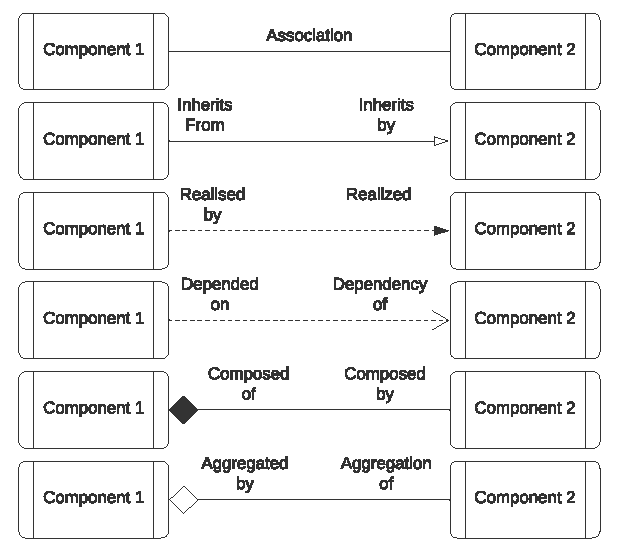
\includegraphics[width=0.4\textwidth]{figures/legenda.pdf}
  \caption[UML Notation used]{UML notation}
  \label{fi:class_diagram_relationship_notation}
\end{figure}

The following sections detail the requirements specific to each element.

\begin{figure*}[ht!]
    \centering
    \centerline{\includegraphics[width=\textwidth]{figures/generic_design.pdf}}
    \caption[Generic architecture]{The Generic architecture of the artifacts}
    \label{fig_design}
\end{figure*}

The ViewModel consists of data attributes representing fields from the corresponding
Entity and may also contain information specific to the user interface. It is important to
note that the ViewModel has no external dependencies on other objects within the
architecture.

The Presenter is derived from the IPresenter interface and adheres to the specified
implementation, which is located in the Application layer. Its main responsibility is to
create the Controller's Response by instantiating the ViewModel, constructing the HTTP
Response message, or combining both as necessary. When needed, the Presenter utilizes the
IMapper interface without depending on specific implementations of IMapper. The Presenter
has an internal scope and cannot be instantiated outside the Presentation layer.

The ViewModelMapper, derived from the IMapper interface, follows the specified
implementation found in the Application layer. Its primary role is to map the necessary
data attributes from the ResponseModel to the ViewModel. The ViewModelMapper also has an
internal scope, ensuring it cannot be instantiated outside the Presentation layer.

The Controller is responsible for receiving external requests and forwarding them to the
appropriate Boundary within the Application layer. It relies on the IBoundary interface
without depending on specific implementations of this interface.

The IBoundary interface establishes the contract for its derived Boundary implementations,
and it has public scope within the system. Boundary implementations, derived from the
IBoundary interface, ensure separation between the internal aspects of the Application
Layer and the other layers. Each Boundary implementation handles a single task, executed
using the IInteractor interface. These implementations also have an internal scope and
cannot be instantiated outside the Application layer.

The IInteractor interface defines the contract for its derived Interactor implementations.
Like Boundary implementations, Interactors have an internal scope and are limited to the
Application layer. Interactor implementations execute single tasks or orchestrate a series
of tasks. Tasks dependent on infrastructure components, such as databases, are handled
through a Gateway. Additionally, Interactor implementations utilize the IMapper interface
to handle mapping between RequestModels, Entities, and ResponseModels.

The IMapper interface establishes the contract for Mapper implementations and has public
scope within the system. Derived from IMapper, the RequestModelMapper is responsible for
mapping the necessary data attributes from the RequestModel to an Entity. The
RequestModelMapper has internal scope and cannot be instantiated outside the Application
layer.

Similarly, the ResponseModelMapper is responsible for mapping data attributes from the
ResponseModel and follows the same implementation and scope restrictions as the
RequestModelMapper.

The IPresenter interface establishes the contract for Presenter implementations, typically
within the Presentation layer. It has public scope and ensures consistency in Presenter
behavior throughout the system.

The Gateway establishes the contract for interaction with infrastructure technologies such
as databases or filesystems. Each Gateway follows a specific naming convention, with
interfaces like ICreateGateway, IGetGateway, IGetByIdGateway, IUpdateGateway and
IDeleteGateway, representing different CRUD operations. Gateway implementations are derived
from these interfaces and are responsible for task-specific interactions with
infrastructure components. These implementations have internal scope and cannot be
instantiated outside their respective layers.

The ResponseModel consists of data attributes representing fields from the corresponding
Entity and may include output-specific data for the Interactor. The ResponseModel does not
depend on external objects within the architecture.

The RequestModel is similarly structured, consisting of data attributes from the
corresponding Entity and input-specific data for the Interactor. It, too, does not depend
on external objects within the architecture.

Data Entities represent corresponding data fields and do not rely on external objects.
They are only utilized by the Application layer.

The Gateway Implementation derives from the corresponding Gateway interface and adheres to
the specified implementation. It is responsible for handling tasks associated with its
infrastructure technology, such as interaction with a SQL database or filesystem. Gateway
Implementations have internal scope and cannot be instantiated outside their respective
layers.

Lastly, each architectural pattern adheres to at least one of the SOLID principles,
ensuring compliance and avoiding violations of these design principles.

\subsection{Expander Requirements} \label{expander_framework_requirements}

In addition to the more generic requirements outlined in previous sections, the following
requirements are specific to the Clean Architecture Expander and Expander Framework
artifact.

The Expander Framework facilitates interaction with the Clean Architecture Expander via a
command-line interface (CLI), which is implemented in the Presentation layer of the
framework. Additionally, the Expander Framework retrieves models from a Microsoft SQL
Server (MSSQL) database using EntityFramework ORM technology, integrated within the
Infrastructure layer. The framework also supports loading and executing configured
Expanders, though in this particular research, only the Clean Architecture Expander is
applied.

Moreover, the Expander Framework supports generic harvesting and injection
functionalities, which can be extended or used by the Expanders in accordance with the
Open-Closed Principle (OCP). This extensibility is further enhanced by the framework's
support for generic template handling, also designed to be extended by the Expanders
following the OCP. The framework adheres to the component and software requirements
outlined in Sections \ref{component_requirements} and \ref{software_requirements} of this
chapter.

The Clean Architecture Expander specifically generates a C\# .NET 7.0 RESTful service,
which provides an HTTP interface atop the Expander Framework’s meta-model, enabling basic
Create, Read, Update, Delete (CRUD) operations. This expander consists solely of an
Application layer and reuses the Domain layer provided by the Expander Framework.
Additionally, the Clean Architecture Expander adheres to the component and software
requirements set forth in Sections \ref{component_requirements} and
\ref{software_requirements} of this chapter.

By adhering to these requirements, both the Expander Framework and the Clean Architecture
Expander align with the overall architecture goals while maintaining flexibility and
extensibility.

\subsubsection{Generated Artifact Requirements} \label{generated_artifact_requirements}

The generated artifact adheres to this chapter's component and software requirements
specified in Sections \ref{component_requirements} and \ref{software_requirements}.


% Chapter 6
\section{The Research Artifacts}

\begin{figure*}[ht!]
  \centering
  \centerline{\includegraphics[scale=0.6]{figures/artifactOverview.pdf}}
  \caption[Schematic overview of the artifacts]{Schematic overview of the artifacts}
  \label{fig_overview_design}
\end{figure*}

The first artifact consists of two main components: the Clean Architecture Expander and
the Expander framework. The name of the Expander Framework, Pantha Rhei, was inspired by
the Greek philosopher \emph{Heraclitus}, who famously stated that \enquote{life is flux.}
The name reflects the artifact's perceived ability to cope with constant change in a
stable and evolvable manner. Users can interact with the Expander Framework using the
\gls{cli} command \enquote*{flux} in combination with several parameters.

As illustrated in Figure \ref{fig_overview_design}, the main task of the first artifact or
\enquote*{expand} the second artifact. By entering the correct command, the Expander
Framework loads the model being instantiated during the expansion process. Then, the
required expanders are prepared based on information available through the model. In the
case of this study, the Clean Architecture Expander. The Clean Architecture Expander
consists of a set of tasks and templates. When the Expander Framework executes the Clean
Architecture Expander, the model is instantiated into the generated artifact with the aid
of the templates.

The model is an instance of the meta-model. Consequently, the model can represent any
application as long as the meta-model is respected. In the case of this study, the model
represents the entities, attributes, relationships, and other characteristics of the
meta-model.

As a result, the second artifact (artifact II) allows a user to modify or maintain the
model used by the Expander Framework by exposing a Restful interface. This method
approaches the meta-circularity process, where an expansion process is used to update the
meta-model. Although not fully compliant with the theory of \gls{ns}, the Expander
Framework consists of the required tasks to update its own meta-model. This is illustrated
in Figure \ref{fig_overview_design} by the \enquote*{updates} arrow.




\input{content/chapter6/name}
\subsection{The Meta-Model and Model} \label{sec_artifact_meta_model}

The meta-model is a blueprint that describes a software system's structure, entities,
relationships, and expanders. The model is an instantiation of the meta-model,
representing a specific software system with unique characteristics. 

Figure \ref{fig_erd} illustrates the version of the meta-model used for this research. A
detailed description of each of the elements can be found in the thesis of
\citeauthor{koks_convergence_2023} \cite[73]{koks_convergence_2023}.

\begin{figure*}[ht!]
    \centering
    \centerline{\includegraphics[scale=0.6]{figures/erd.pdf}}
    \caption[The meta-model represented as an Entity Relationship Diagram]{The meta-model represented as an Entity Relationship Diagram}
    \label{fig_erd}
\end{figure*}
\subsection{Plugin Architecture} \label{subsec_plugin_architecture}

The Expander Framework artifact is responsible for loading and bootstrapping Expanders and
initiating the generation process. Expanders are dynamically loaded at runtime through a
dotnet capability called assembly binding, allowing the architecture illustrated in the
following image \parencite{koks_expanderpluginloaderinteractor_2023}.

\begin{figure}[htbp]
  \centering
  \includegraphics[width=0.5\textwidth]{figures/plugin_architecture.pdf}
  \caption[Plugin Archticture]{Expanders are considered plugins}
  \label{fi:plugin_architecture}
\end{figure}

This plugin design adheres to several principles of \gls{solid}. The \gls{srp} principle
is implemented by ensuring that an Expander generates one and only one construct. The
\gls{ocp} principle is applied by allowing the creation of new expanders in addition to
the already existing ones. The \gls{lsp} principle is respected by enabling the addition
or replacement of expanders without modifying the internal workings of the Expander
Framework.
\subsection{Expanders}

The Exander Framework allows for the miscellaneous execution of expanders of any type. The
Expander Framework is independent of any of the details of Expanders, fully adhering to
the principle of \gls{dip}. Conversely, an Expander is required to implement several
interfaces to ensure execution and dependency management are available during runtime. The
Expander Framework also consists of a set of default tasks, such as the execution of the
expansion tasks known as ExpanderHandlerInteractors
\citecode{koks_iexpanderhandlerinteractor_2023}, logging, bootstrapping dependencies, and
tasks to execute harvestings and injections. Except for the use of the
IExpanderInteractor, non of which are required.

Figure \ref{fig_expander_design} illustrates the dependencies between the domain layer of
the Expander Framework. The Clean Architecture Expander is considered an application layer
containing specific tasks bounded to a particular application or process. In this case,
the Expansion process.

\begin{figure*}[htbp]
    \centering
    \includegraphics[width=1\textwidth]{figures/expander.pdf}
    \caption[The design of an Expander]{The design of an Expander}
    \label{fig_expander_design}
  \end{figure*}
\subsection{Executing Commands} \label{subsec_IExecutionInteractorObject}

An exciting implementation that facilitates a high degree of cohesion while maintaining
low coupling is the utilization of the \code{koks_iexecutioninteractor_2023} interface
\parencite{koks_iexecutioninteractor_2023}. This interface allows for the execution of
various derived types responsible for various tasks, such as executing Handlers,
Harvesters, and Rejuvenators\footnote{It is important to note that the Rejuvenation
objects in this version of the artifact are capable of performing injections and not the
entire Rejuvenation process.} \parencites{koks_expandentitieshandlerinteractor_2023,
koks_regionharvesterinteractor_2023, koks_regionrejuvenatorinteractor_2023}. The
implementation promotes decoupling by adhering to both \gls{ocp} and \gls{lsp}.

\begin{figure*}[htbp]
    \centering
    \includegraphics[width=1\textwidth]{figures/command_pattern.pdf}
    \caption[Low coupling with \code{koks_iexecutioninteractor_2023}]{Low coupling with \code{koks_iexecutioninteractor_2023}}
    \label{fig_iexecutioninteractor}
  \end{figure*}


Figure \ref{fig_iexecutioninteractor} illustrates that the required interfaces are placed
in the Domain layer of the Expander Framework. In contrast, the concrete classes also can
be implemented as part of the internal scope of the Clean Architecture Expander
\parencite{koks_migrationharvesterinteractor_2023}. Code listing
(((REPLACE CODE LISTING))) illustrates an implementation example of
this interface. Finally, the code listing (((REPLACE CODE LISTING)))
illustrates the aggregation of the execution, which allows for a graceful cohesion of the
execution Tasks \parencite{koks_codegeneratorinteractor_2023}.

\subsection{Dependency Management}

Dependency management is an extremely valuable aspect of achieving stability and
evolvability. Dependency management can be achieved by using Dependency Injection. This
research acknowledges \textcite[215]{mannaert_normalized_2016} statement that Dependency
Injection does not solve coupling between classes. Working on the artifact has shown that
combinatorial effects can occur when not careful. Nevertheless, Dependency Injection is a
widely used pattern in building the artifact. In order to achieve stability and
evolvability, the Dependency Injection pattern \underline{must} be combined with various
other principles of both \gls{ca} and \gls{ns}. 

The goal is to centralize the management of dependencies and remove unwanted manual object
instantiations in the code; al this while respecting the \gls{dip} principle so that each
component layer is responsible for managing its dependencies. The artifact achieves this
by using extension methods \parencite{koks_dependencyinjectionextension_2023}. Additionally, and quite significantly,
implementations primarily rely on abstractions or contracts (interfaces) instead of the
details of concrete implementations. 

Traditionally, Dependency Injection injects instantiations through constructor parameters
or class properties. Although there are benefits in this approach, doing so will
eventually lead to combinatorial effects, breaking the stability of a software artifact.
In order to solve this problem, the artifact used the Service Locator pattern, a central
registry responsible for resolving dependencies \parencite{wikipedia_service_2023}. Many 
frameworks are available from \gls{nuget}, but the artifact uses the Service Registry,
which is part of the .NET framework. This service registry is considered a cross-cutting
concern. The dependency on this technology is reduced by applying the principles of the
\gls{lsp} and \gls{isp}. The artifact creates and uses separate interfaces to register
\parencite{koks_idependencymanagerinteractor_2023} and resolve
\parencite{koks_idependencyfactoryinteractor_2023} dependencies. The framework technology
dependencies are abstracted behind implementing those interfaces
\parencite{koks_dependencymanagerinteractor_2023}. 

The approach described here has many advantages in managing the stability and evolvability
of the software artifact. However, as for most things, there are also some drawbacks. For
example, a good amount of experience is required for developers to understand code that
incorporates abstractions, contracts, and Dependency Injection. Another drawback is that
dependency errors are detected in runtime rather than compile time. The benefits of the
artifacts, however, outweigh the drawbacks.

\section{conclusion}

The primary objective of \citename{koks_convergence_2023}{author} was to study the
convergence between \gls{ca} and \gls{ns} by analyzing their principles and design
elements through theory and practice. This section will summarize the findings into a
research conclusion.

A noteworthy distinction between \gls{ns} and \gls{ca} lies in their foundational roots.
\gls{ns} is a product of computer science research built upon formal theories and
principles derived from rigorous scientific investigation. Throughout this
paper, \gls{ns} is referred to as a development approach or paradigm, it is actually a
part of Computer Science.

Stability and evolvability are concepts not directly referenced in the literature on
\gls{ca}, but this design approach aligns with the goal of \gls{ns}. The attentive reader
can observe the shared emphasis on modularity and the separation of concerns, as all SOLID
principles strongly converge with \gls{soc}. Both approaches attempt to achieve low
coupling and high cohesion. In addition, \gls{ca} adds the dimensions of dependency
management as useful measures to improve maintainability by rigorously managing
dependencies in the Software Architecture.

The \gls{dvt} appears to be underrepresented in the SOLID principles of \gls{ca}.
\gls{dvt} is primarily supported by the \gls{srp} of \gls{ca}, as evidenced by ViewModels,
RequestModels, ResponseModels, and Entities as software elements. It is worth noting that
this application of Data Version Transparency  is an integral part of the design elements
of \gls{ca}. While \gls{ca} does address \gls{dvt} through the \gls{srp}, a more
comprehensive representation of the underlying idea of \gls{dvt} within the principles of
\gls{ca} will likely improve the convergence of \gls{ca} with \gls{ns}.

The underrepresentation of \gls{dvt} has led to significant combinatorial effects in some
parts of the researcher's artifacts. These combinatorial effects might be attributed to the
author's inexperience in creating systems that enable code generation through expansion
while maintaining stability on templates and craftings. If \gls{dvt} were better
represented in the principles of \gls{ca}, the severity of the combinatorial effects would
have most likely been less.

\gls{ca} Lacks a strong foundation for receiving external triggers in its design
philosophy. This is partially represented by the Controller element. However, this element
is described as being used for web-enabled environments and might result in a less
comprehensive approach to receiving external triggers across various technologies or
systems.

The most notable difference between \gls{ca} and \gls{ns} is their approach to handling
state. \gls{ca} does not explicitly address state management in its principles or design
elements. \gls{ns} Provides the principle of \gls{sos}, ensuring that state changes within
a software system are stable and evolvable. This principle can be crucial in developing
scalable and high-performance systems, as it isolates state changes from the rest of the
system, reducing the impact of state-related dependencies and side effects. 

The findings can only lead to the conclusion that the convergence between \gls{ca} and
\gls{ns} is incomplete.  Consequently, \gls{ca} cannot fully ensure stable and evolvable
software artifacts as \gls{ns} has defined them.

While it has been demonstrated that the convergence between these two approaches is
incomplete, combining both methodologies is highly beneficial for \gls{ns} and \gls{ca}
for various reasons. The primary advantage of synergizing them lies in the complementary
nature of both paradigms, where each approach provides strengths that can be leveraged to
address a robust architectural design. 

\gls{ca} offers a well defined, practical, and modular structure for software development.
Its principles, such as SOLID, guide developers in creating maintainable, testable, and
scalable systems. This architectural design approach is highly suitable for various
applications and can be easily integrated with the theoretical foundations provided by
\gls{ns}. Conversely, the \gls{ns} approach offers a more comprehensive theoretical
understanding of achieving stable and evolvable systems. 

To conclude, the popularity and widespread adoption of \gls{ca} in the software
development community can benefit \gls{ns}. As more developers adopt \gls{ca}, they become
more familiar with \gls{ns} and recognize their value to software design. Synergizing both
approaches will likely lead to increased adoption of \gls{ns}.

\printbibliography[heading=bibintoc, keyword={bib}, title=Bibliography]
\printbibliography[heading=bibintoc,  keyword={artifact}, title=Code Samples]
% %\include{content/glossaries}

\end{document} 
 